\hypertarget{apr__want_8h}{}\section{/usr/local/src/github/\+Codebase/httpd-\/2.4.29/srclib/apr/include/apr\+\_\+want.h File Reference}
\label{apr__want_8h}\index{/usr/local/src/github/\+Codebase/httpd-\/2.\+4.\+29/srclib/apr/include/apr\+\_\+want.\+h@{/usr/local/src/github/\+Codebase/httpd-\/2.\+4.\+29/srclib/apr/include/apr\+\_\+want.\+h}}


A\+PR Standard Headers Support.  


{\ttfamily \#include \char`\"{}apr.\+h\char`\"{}}\\*
{\ttfamily \#include $<$string.\+h$>$}\\*
Include dependency graph for apr\+\_\+want.\+h\+:
\nopagebreak
\begin{figure}[H]
\begin{center}
\leavevmode
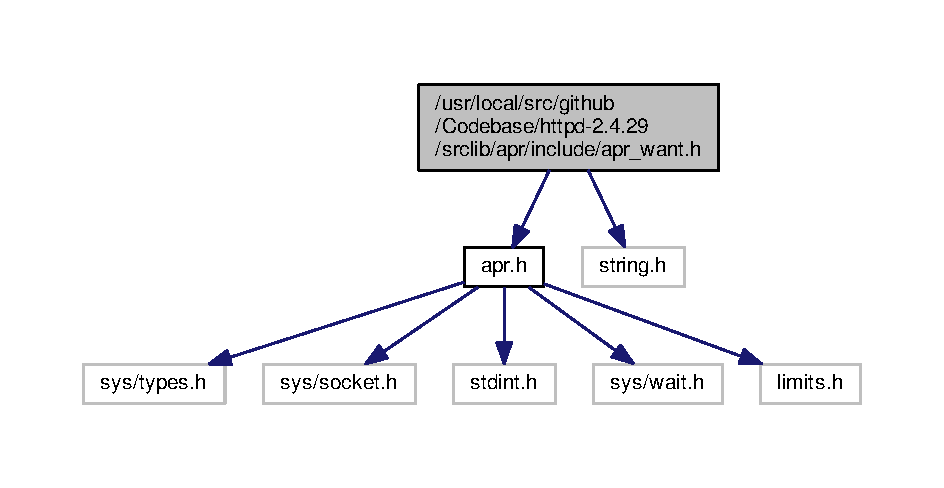
\includegraphics[width=350pt]{apr__want_8h__incl}
\end{center}
\end{figure}


\subsection{Detailed Description}
A\+PR Standard Headers Support. 


\begin{DoxyPre}
Features:\end{DoxyPre}



\begin{DoxyPre}  APR\_WANT\_STRFUNC:  strcmp, strcat, strcpy, etc
  APR\_WANT\_MEMFUNC:  memcmp, memcpy, etc
  APR\_WANT\_STDIO:    <stdio.h> and related bits
  APR\_WANT\_IOVEC:    struct iovec
  APR\_WANT\_BYTEFUNC: htons, htonl, ntohl, ntohs\end{DoxyPre}



\begin{DoxyPre}Typical usage:\end{DoxyPre}



\begin{DoxyPre}  \#define APR\_WANT\_STRFUNC
  \#define APR\_WANT\_MEMFUNC
  \#include "apr\_want.h"\end{DoxyPre}



\begin{DoxyPre}The appropriate headers will be included.\end{DoxyPre}



\begin{DoxyPre}Note: it is safe to use this in a header (it won't interfere with other
      headers' or source files' use of apr\_want.h)
\end{DoxyPre}
 